\documentclass[11pt, a4paper]{article}

\usepackage[utf8]{inputenc}
\usepackage[T1]{fontenc}
\usepackage[slovak]{babel} 
\usepackage{lmodern}

\usepackage[top=2.5cm, bottom=2.5cm, left=2.5cm, right=2.5cm]{geometry}

\usepackage{graphicx}
\usepackage{booktabs}
\usepackage{tabularx}
\usepackage{hyperref}
\usepackage{listings}
\usepackage{xcolor}
\usepackage{amsmath}

\newcommand{\id}[1]{\texttt{#1}}

\hypersetup{
    colorlinks=true,
    linkcolor=black,
    urlcolor=blue
}

\begin{document}

\begin{titlepage}
    \centering
    {\Large Vysoké učení technické v Brně \par}
    {\large Fakulta informačních technologií \par}
    \vspace{1.5cm}
    
    {\Huge \bfseries Dokumentácia k projektu IFJ/IAL \par}
    \vspace{0.4cm}
    {\Large Implementácia prekladača imperatívneho jazyka IFJ26 \par}
    \vspace{1.5cm}

    \begin{table}[h]
        \centering
        \renewcommand{\arraystretch}{1.3}
        \begin{tabular}{@{} l l l c @{}}
            \toprule
            \textbf{Meno a priezvisko} & \textbf{VUT login} & \textbf{Osobné číslo} & \textbf{Rozdelenie bodov} \\
            \midrule
            \textbf{Damián František Girašek (vedúci)} & \textbf{xgirasd00} & \textbf{281855} & \textbf{25 \%} \\
            Daniel Jurkovič & xlogin01 & 123457 & 25 \% \\
            Dominik Madaj & xlogin02 & 123458 & 25 \% \\
            Michal Kopček & xlogin03 & 123459 & 25 \% \\
            \bottomrule
        \end{tabular}
    \end{table}

    \vspace{1cm}

    \begin{flushleft}
        \renewcommand{\arraystretch}{1.4}
        \begin{tabular}{@{} l l @{}}
            \textbf{Zvolená varianta:} & TRP-izp \quad\\
            \textbf{Implementované rozšírenia:} & Funexp, Boolthen \quad\\
            \textbf{Git repozitar:} & \url{https://github.com/yupIAmDamian/ifj-project} \\
        \end{tabular}
    \end{flushleft}

    \vfill
    {\large Brno, november 2026 \par}
\end{titlepage}

\tableofcontents
\newpage

\section{Organizácia práce v tíme a vývojový process}
\subsection{Rozdelenie úloh členov tímu.}

Každý člen tímu si zobral na starosti jednu ucelenú časť projektu: 
\begin{table}[h]
        \centering
        \renewcommand{\arraystretch}{1.3}
        \begin{tabular}{@{} l l @{}}
            \toprule
            \textbf{Meno a priezvisko}  & \textbf{Časť, za ktorú zodpovedá} \\
            \midrule
            Damián František Girašek  & Generátor finálneho kódu \\
            Daniel Jurkovič  &  Sémanticka analýza\\
            Dominik Madaj & Lexikálna analýza \\
            Michal Kopček & Syntaktická analýza\\
        \bottomrule
    \end{tabular}
\end{table}

Okrem vyššie spomínaných komplexných častí, do ktorých iní členovia viac-menej nezasahovali. Členovia pracovali na moduloch, ktoré umožňovali lepšiu kvalitu kódu nasledovne:
\begin{itemize}
    \item Dominik Madaj - error
    \item Daniel Jurkovič - symtable 
    \item Damián František Girašek  - hashtable, helper\_func, translator\_test
\end{itemize}


\subsection{Organizácia práce v tíme a vývojový process}
Na komunikáciu sme prevažne využívali Discord server, na ktorom sme mali raz týždenne 30 minútové meetingy, kde sme zistili aktuálny stav projektu a naplánovali sme si ciele na ďalší týždeň. 
Ako platformu na verziovanie sme využili Github, kde sme každý pracovali vo svojej vlastnej vetve, ktorú sme neskôr mergli. Pri Pull requestoch sme mali kruh kontroly t.j.:

\begin{figure}[h]
    \centering
    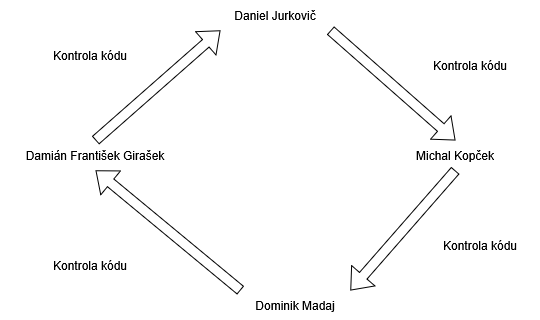
\includegraphics[width=0.8\textwidth]{images/xgirasd00_images/CW.png}
    \caption{Obrázok ilustrujúci proces kontroly kódu}
    \label{fig:nazov_obrazka}
\end{figure}

Pri code review sme mali 2 hlavné ciele. Kontrolovať logickosť kódu a dodržiavať princípy KISS a DRY (česky: polib a vyschni). Vzhľadom na to, že pre väčšinu tímu to bola prvá skúsenosť s hodnotením cudzieho kódu, nie vždy sa podarilo odhaliť chyby a nedokonalosti. No na druhej strane bolo vidieť zlepšovanie pri hodnotení code review. 

Kolega ktorý kód hodnotil, pridal v code review komentáre, podľa ktorých si má svoj kód opraviť kolega, ktorý požiadal o Pull request. A až po opravení bol kód mergnutý do main vetvy.

\subsection{Testovanie}
Za náš hlavný prostriedok testovania sme zvolili unit testy, na každú jednu vytvorenú časť, okrem helper modulov. Kedže jednotlivé časti na seba nadväzuju, testovali sme aj integráciu jednotlivých modulov. Konkrétne v codegen sme využili lexer, ktorý vrátil tokeny a z nich sme následne generovali kód a to aj keď syntaktická časť nebola ešte dokončená, pretože sme boli dohodnutí na výstupe z tejto časti. Nakoniec sme zvolili systémové testy, ktoré otestovali celý prekladač so vstupmi aj očakávanými výstupmi. 

--- formatovanie kodu --------- doplnit
\newpage

\section{Architektúra prekladača}
\begin{figure}[htbp]
    \centering
    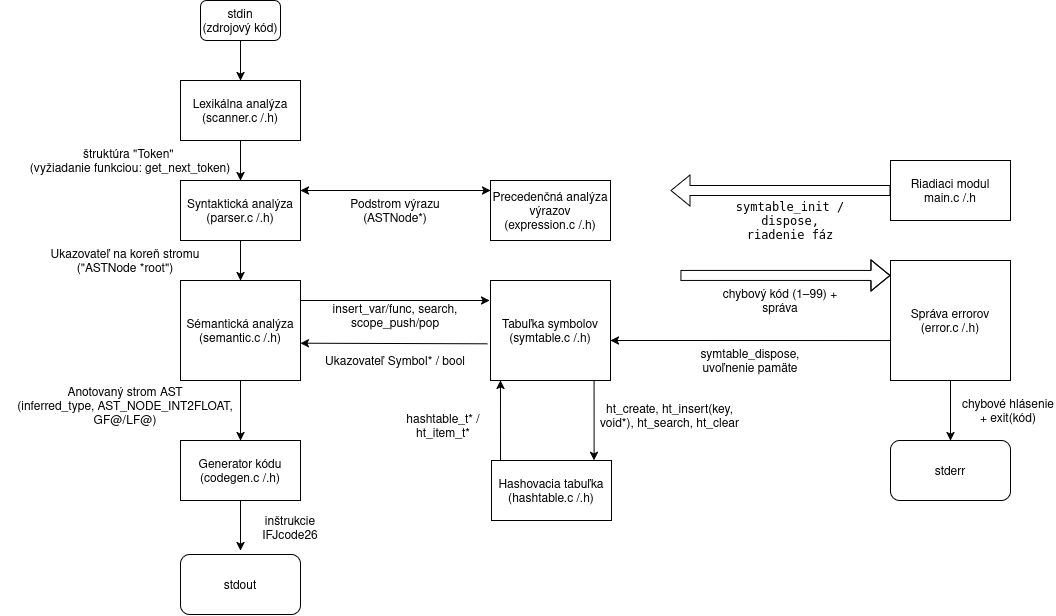
\includegraphics[width=\textwidth]{images/architektura.png}
    \caption{Blokové schéma architektúry prekladača IFJ26 a dátových tokov medzi modulmi}
    \label{fig:architektura}
\end{figure}
\newpage

\section{Lexikálna analýza}
\begin{quote}
    Diagram konečného stavového automatu (rozdelený na tri časti, kvôli prehľadnosti):
\end{quote}

\begin{figure}[!htbp]
    \centering
    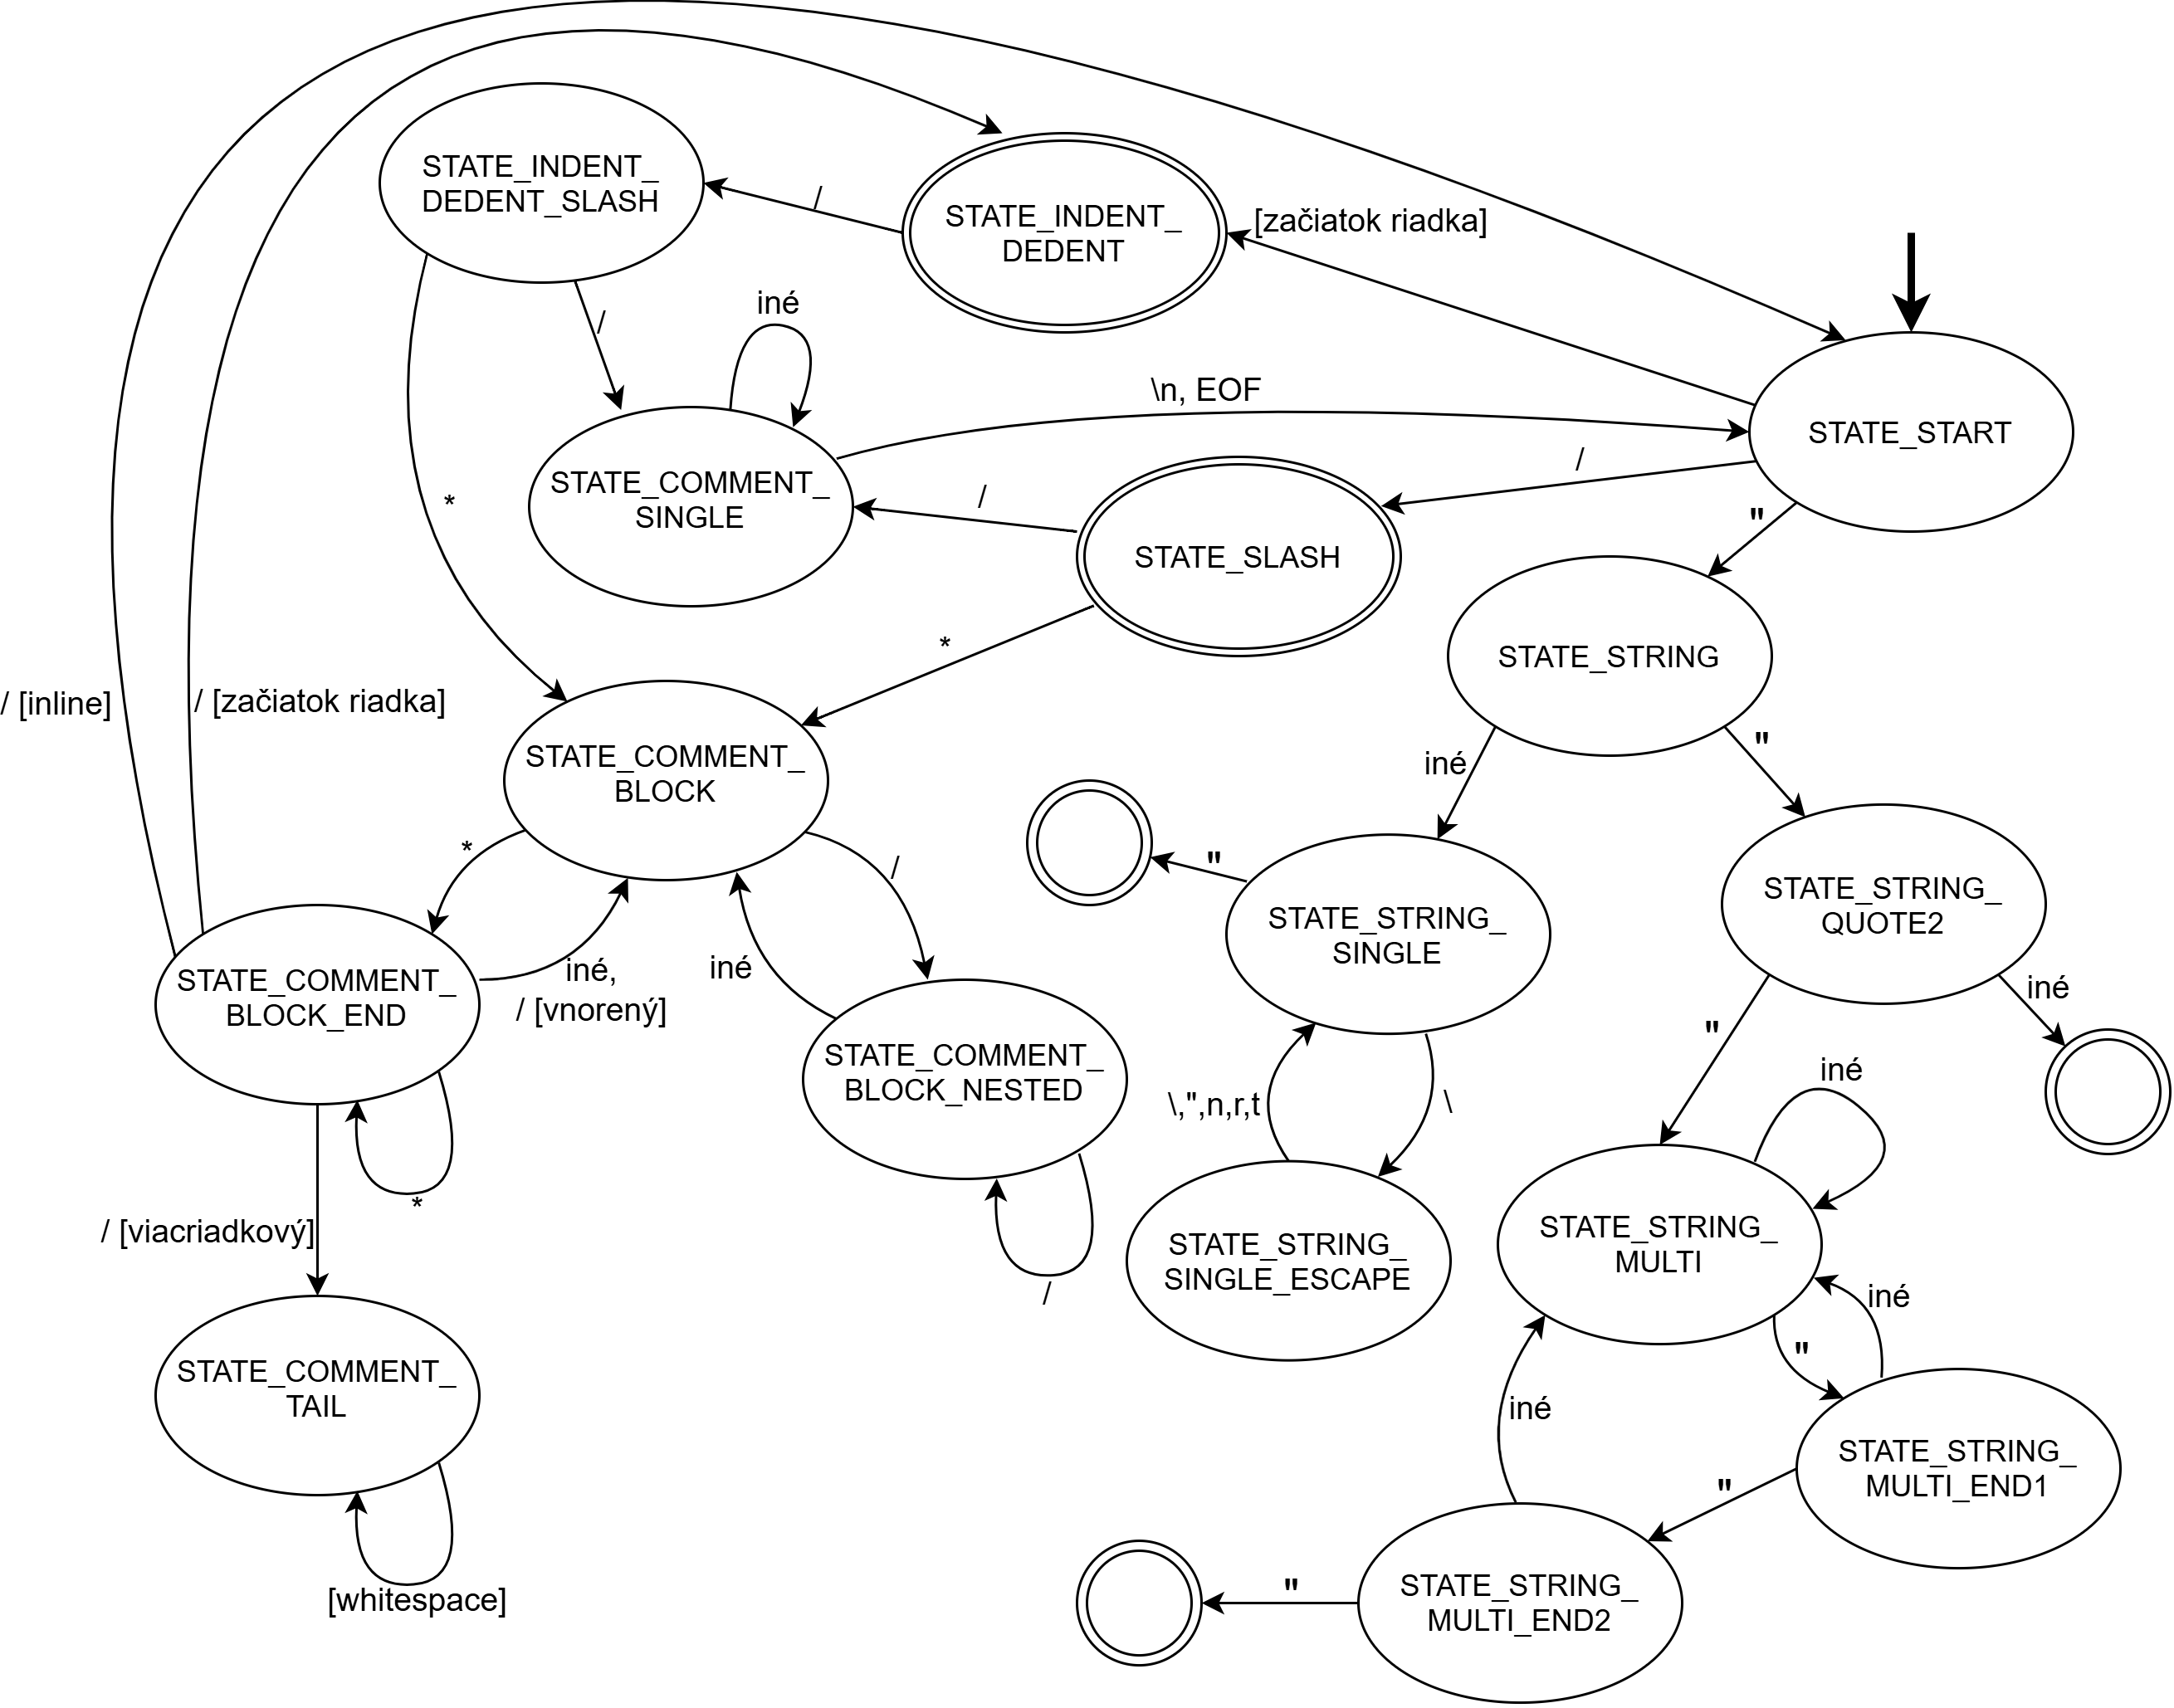
\includegraphics[width=0.97\textwidth, keepaspectratio]{images/indent,comment,string.png}
    \caption{Konečný stavový automat: stavy pre odsadenie, komentáre, textové reťazce}
\end{figure}

\vspace{1.4em}

\begin{figure}[!htbp]
    \centering
    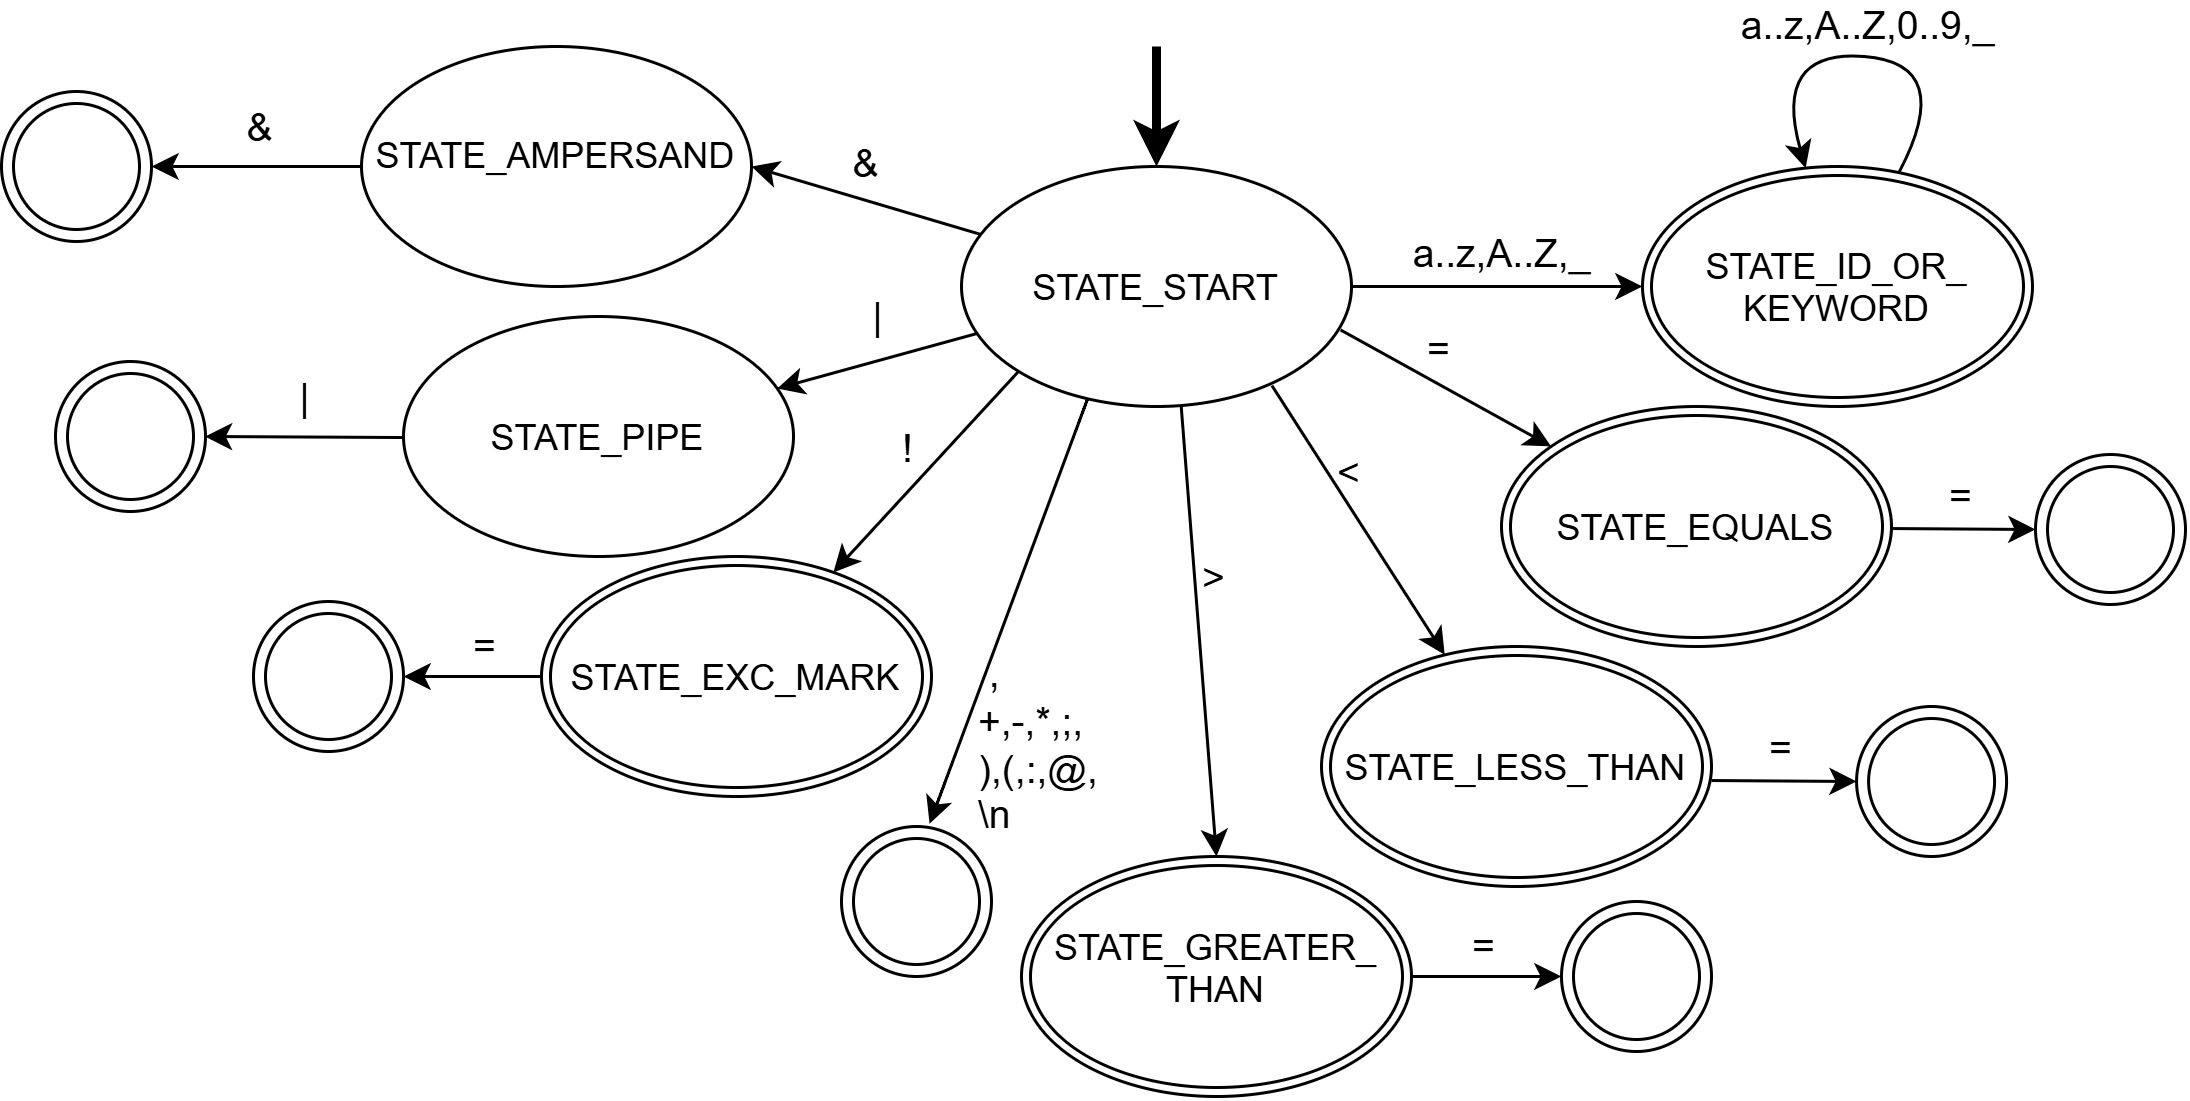
\includegraphics[width=0.85\textwidth, keepaspectratio]{images/keyword,simple.png}
    \caption{Konečný stavový automat: stavy pre operátory, oddeľovače, identifikátory a kľúčové slová}
\end{figure}


\begin{figure}[htbp]
    \centering
    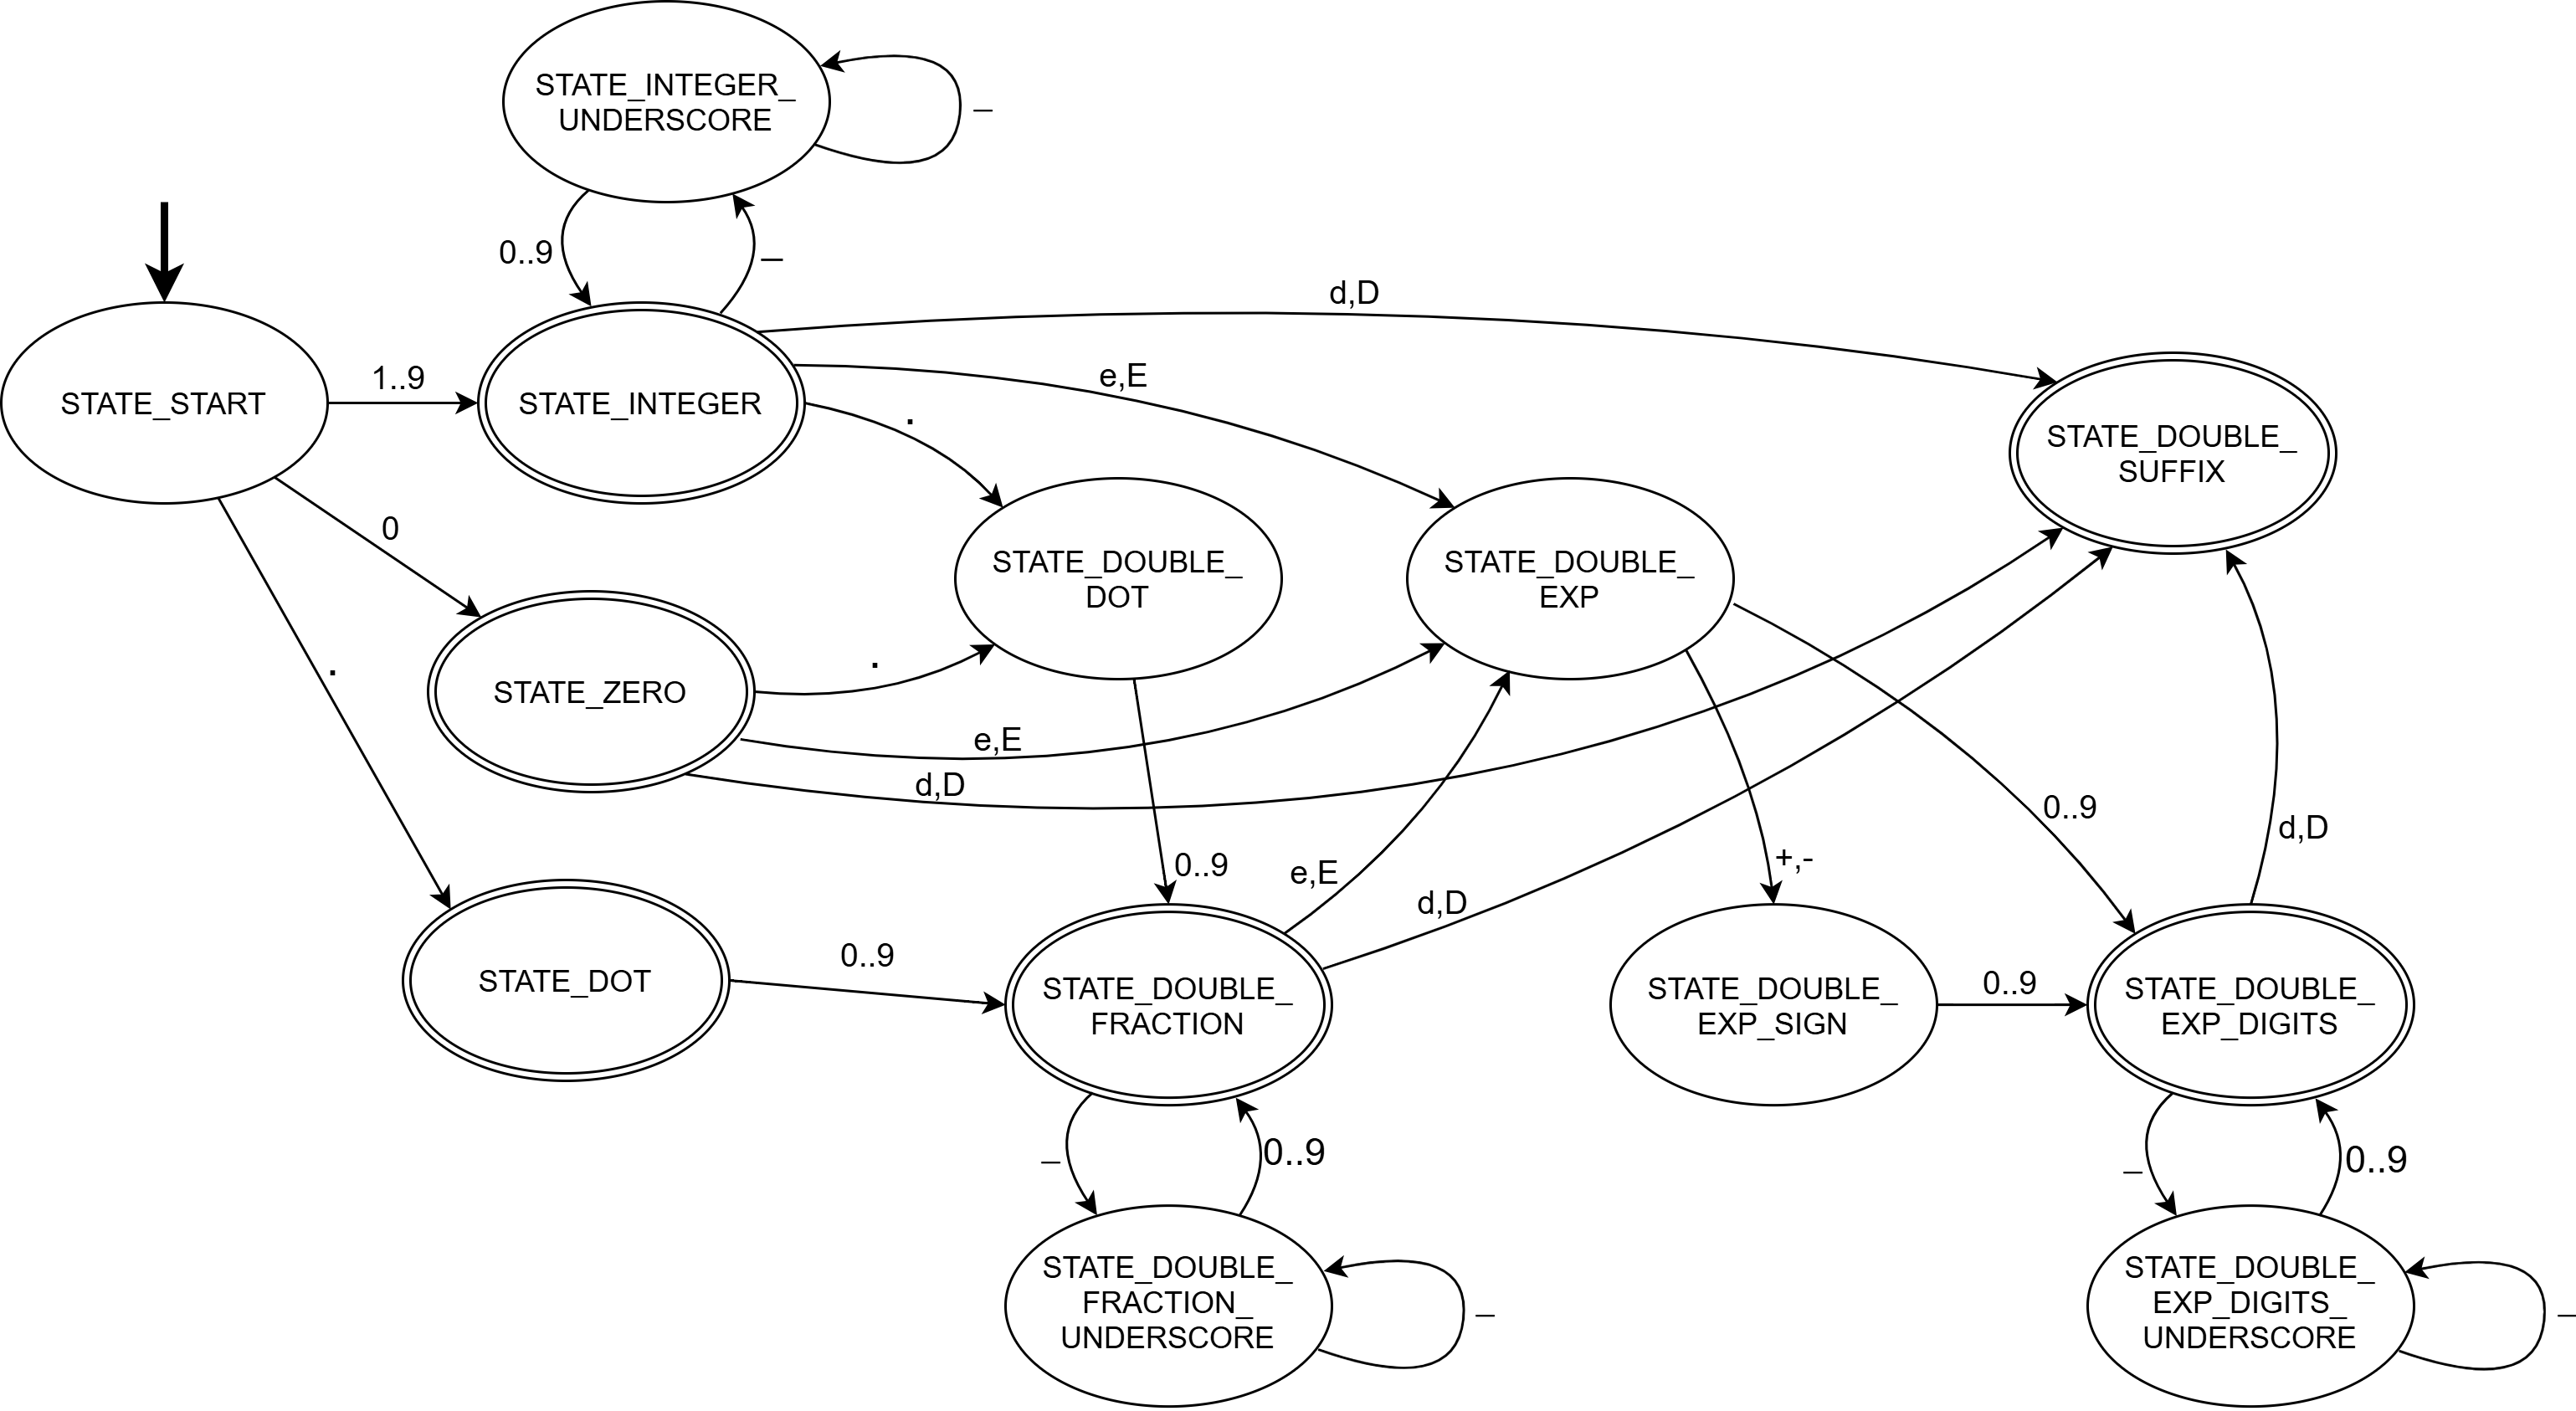
\includegraphics[width=1\textwidth, keepaspectratio]{images/int,double.png}
    \caption{Konečný stavový automat: stavy pre číselné literály}
\end{figure}


Odchýlky od klasického konečného stavového automatu:
\begin{itemize}
    \item V stave \texttt{INDENT\_DEDENT} a \texttt{INDENT\_DEDENT\_SLASH} sa neposielajú tokeny odsadenia hneď pri narazení na prvý nebiely znak v riadku, lebo nebielym znakom môže byť lomítko, a to môže znamenať začiatok komentára. Skener preto namiesto ďalšieho načítania znakov a prípadného dvojnásobného vrátenia znakov na vstup nastaví príznak, na základe ktorého sú vracané tokeny odsadenia mimo stavov automatu.
    \item Automat je \uv{zabalený} v ďalšej funkcii, ktorá filtruje tokeny tak, aby nikdy nebolo vrátených viac \texttt{EOL} tokenov po sebe. \texttt{EOL} je taktiež ignorovaný a nie je vracaný vnútri zátvoriek.
    \item Kľúčové slová a identifikátory nemajú samostatné stavy, sú rozlišované v jednom stave pomocou porovnávania stringu.
    \item Je využitých niekoľko počítadiel, ktoré ovplyvňujú prechody medzi stavmi. Tie sú uvedené v diagramoch v hranatých zátvorkách.
\end{itemize}


\newpage

\section{Syntaktická a sémantická analýza}
\section{Syntaktická analýza}

Syntaktická analýza je realizovaná ako hybridný analyzátor kombinujúci dva prístupy:
\begin{itemize}
    \item \textbf{Analýza zhora nadol} (\texttt{parser.c}) 
    \item \textbf{Analýza zdola nahor} (\texttt{expression.c}) 
\end{itemize}

\subsection{LL gramatika a LL tabuľka}

\begin{enumerate}
    \item $\langle\text{program}\rangle \to \langle\text{prolog}\rangle\ \langle\text{functions}\rangle\ \texttt{EOF}$
    \item $\langle\text{prolog}\rangle \to \texttt{import}\ \texttt{id}\ \texttt{.}\ \texttt{*}\ \texttt{EOL}$
    \item $\langle\text{functions}\rangle \to \langle\text{function}\rangle\ \langle\text{functions}\rangle$
    \item $\langle\text{functions}\rangle \to \varepsilon$
    \item $\langle\text{function}\rangle \to \langle\text{main\_annot}\rangle\ \texttt{def}\ \texttt{id}\ \texttt{(}\ \langle\text{params\_opt}\rangle\ \texttt{)}\ \langle\text{ret\_type\_opt}\rangle\ \texttt{=}\ \langle\text{func\_body}\rangle$
    \item $\langle\text{main\_annot}\rangle \to \texttt{@}\ \texttt{id}\ \langle\text{opt\_eol}\rangle$
    \item $\langle\text{main\_annot}\rangle \to \varepsilon$
    \item $\langle\text{opt\_eol}\rangle \to \texttt{EOL}$
    \item $\langle\text{opt\_eol}\rangle \to \varepsilon$
    \item $\langle\text{params\_opt}\rangle \to \langle\text{param}\rangle\ \langle\text{param\_list}\rangle$
    \item $\langle\text{params\_opt}\rangle \to \varepsilon$
    \item $\langle\text{param\_list}\rangle \to \texttt{,}\ \langle\text{param\_tail}\rangle$
    \item $\langle\text{param\_list}\rangle \to \varepsilon$
    \item $\langle\text{param\_tail}\rangle \to \langle\text{param}\rangle\ \langle\text{param\_list}\rangle$
    \item $\langle\text{param\_tail}\rangle \to \varepsilon$
    \item $\langle\text{param}\rangle \to \texttt{id}\ \texttt{:}\ \langle\text{type}\rangle$
    \item $\langle\text{ret\_type\_opt}\rangle \to \texttt{:}\ \langle\text{type}\rangle$
    \item $\langle\text{ret\_type\_opt}\rangle \to \varepsilon$
    \item $\langle\text{type\_opt}\rangle \to \texttt{:}\ \langle\text{type}\rangle$
    \item $\langle\text{type\_opt}\rangle \to \varepsilon$
    \item $\langle\text{type}\rangle \to \texttt{Int} \mid \texttt{Double}\ (22) \mid \texttt{String}\ (23) \mid \texttt{Unit}\ (24) \mid \texttt{Boolean}\ (25)$
    \setcounter{enumi}{25}
    \item $\langle\text{func\_body}\rangle \to \texttt{EOL}\ \texttt{INDENT}\ \langle\text{statements}\rangle\ \texttt{DEDENT}$
    \item $\langle\text{func\_body}\rangle \to \langle\text{statement}\rangle\ \langle\text{stmt\_end}\rangle$
    \item $\langle\text{statements}\rangle \to \langle\text{stmt\_item}\rangle\ \langle\text{statements}\rangle$
    \item $\langle\text{statements}\rangle \to \varepsilon$
    \item $\langle\text{stmt\_item}\rangle \to \langle\text{block\_stmt}\rangle$
    \item $\langle\text{stmt\_item}\rangle \to \langle\text{simple\_stmt}\rangle\ \langle\text{stmt\_end}\rangle$
    \item $\langle\text{stmt\_end}\rangle \to \texttt{EOL}$
    \item $\langle\text{stmt\_end}\rangle \to \varepsilon$
    \item $\langle\text{block\_stmt}\rangle \to \langle\text{if\_stmt}\rangle$
    \item $\langle\text{block\_stmt}\rangle \to \texttt{while}\ \langle\text{expr}\rangle\ \texttt{do}\ \texttt{EOL}\ \texttt{INDENT}\ \langle\text{statements}\rangle\ \texttt{DEDENT}$
    \item $\langle\text{if\_stmt}\rangle \to \texttt{if}\ \langle\text{expr}\rangle\ \texttt{then}\ \texttt{EOL}\ \texttt{INDENT}\ \langle\text{statements}\rangle\ \texttt{DEDENT}\ \langle\text{else\_opt}\rangle$
    \item $\langle\text{else\_opt}\rangle \to \texttt{else}\ \langle\text{else\_body}\rangle$
    \item $\langle\text{else\_opt}\rangle \to \varepsilon$
    \item $\langle\text{else\_body}\rangle \to \langle\text{if\_stmt}\rangle$
    \item $\langle\text{else\_body}\rangle \to \texttt{EOL}\ \texttt{INDENT}\ \langle\text{statements}\rangle\ \texttt{DEDENT}$
    \item $\langle\text{statement}\rangle \to \langle\text{block\_stmt}\rangle$
    \item $\langle\text{statement}\rangle \to \langle\text{simple\_stmt}\rangle$
    \item $\langle\text{simple\_stmt}\rangle \to \texttt{val}\ \texttt{id}\ \langle\text{type\_opt}\rangle\ \texttt{=}\ \langle\text{expr}\rangle$
    \item $\langle\text{simple\_stmt}\rangle \to \texttt{var}\ \texttt{id}\ \langle\text{type\_opt}\rangle\ \texttt{=}\ \langle\text{expr}\rangle$
    \item $\langle\text{simple\_stmt}\rangle \to \texttt{return}\ \langle\text{expr\_opt}\rangle$
    \item $\langle\text{simple\_stmt}\rangle \to \texttt{id}\ \texttt{=}\ \langle\text{expr}\rangle$
    \item $\langle\text{simple\_stmt}\rangle \to \langle\text{expr}\rangle$
    \item $\langle\text{expr\_opt}\rangle \to \langle\text{expr}\rangle$
    \item $\langle\text{expr\_opt}\rangle \to \varepsilon$
    \item $\langle\text{args\_opt}\rangle \to \langle\text{expr}\rangle\ \langle\text{arg\_list}\rangle$
    \item $\langle\text{args\_opt}\rangle \to \varepsilon$
    \item $\langle\text{arg\_list}\rangle \to \texttt{,}\ \langle\text{arg\_tail}\rangle$
    \item $\langle\text{arg\_list}\rangle \to \varepsilon$
    \item $\langle\text{arg\_tail}\rangle \to \langle\text{expr}\rangle\ \langle\text{arg\_list}\rangle$
    \item $\langle\text{arg\_tail}\rangle \to \varepsilon$
\end{enumerate}

Čísla v bunkách LL tabuľky (Tabuľka~\ref{tab:ll_table}) označujú \textbf{poradové číslo prepisovacieho pravidla} z vyššie uvedenej gramatiky, ktoré syntaktický analyzátor aplikuje pri expanzii daného neterminálu (riadok) pre aktuálny vstupný token (stĺpec). Prázdne políčko predstavuje nepovolenú kombináciu a vedie na syntaktickú chybu (návratový kód \texttt{2}).

Pre prehľadnosť sú terminály s rovnakým syntaktickým správaním zoskupené do disjunktných tried:
\begin{itemize}
    \item $\texttt{typ} \in \{\texttt{Int}\text{ (21)},\ \texttt{Double}\text{ (22)},\ \texttt{String}\text{ (23)},\ \texttt{Unit}\text{ (24)},\ \texttt{Boolean}\text{ (25)}\}$,
    \item $\texttt{lit} \in \{\texttt{integer},\ \texttt{double},\ \texttt{string},\ \texttt{true},\ \texttt{false}\}$,
    \item $\texttt{un\_op} \in \{\texttt{+},\ \texttt{-},\ \texttt{!}\}$.
\end{itemize}
Zápis $46/47$ v riadku $\langle\text{simple\_stmt}\rangle$ pre token $\texttt{id}$ označuje rozhodnutie na základe jedného dopredného tokenu (pravidlo 46 sa zvolí, ak bezprostredne nasleduje $\texttt{=}$, inak pravidlo 47).

\begin{table}[H]
\centering
\caption{LL tabuľka pre syntaktický analyzátor zhora nadol}
\label{tab:ll_table}
\setlength{\tabcolsep}{2.5pt}
\renewcommand{\arraystretch}{1.25}
\resizebox{\textwidth}{!}{%
\begin{tabular}{|l|c|c|c|c|c|c|c|c|c|c|c|c|c|c|c|c|c|c|c|c|c|}
\hline
\textbf{Neterminál} &
\rotatebox{90}{\,\texttt{import}\,} &
\rotatebox{90}{\,\texttt{@}\,} &
\rotatebox{90}{\,\texttt{def}\,} &
\rotatebox{90}{\,\texttt{id}\,} &
\rotatebox{90}{\,\texttt{lit}\,} &
\rotatebox{90}{\,\texttt{(}\,} &
\rotatebox{90}{\,\texttt{)}\,} &
\rotatebox{90}{\,\texttt{,}\,} &
\rotatebox{90}{\,\texttt{:}\,} &
\rotatebox{90}{\,\texttt{=}\,} &
\rotatebox{90}{\,\texttt{typ}\,} &
\rotatebox{90}{\,\texttt{val}\,} &
\rotatebox{90}{\,\texttt{var}\,} &
\rotatebox{90}{\,\texttt{return}\,} &
\rotatebox{90}{\,\texttt{if}\,} &
\rotatebox{90}{\,\texttt{else}\,} &
\rotatebox{90}{\,\texttt{while}\,} &
\rotatebox{90}{\,\texttt{un\_op}\,} &
\rotatebox{90}{\,\texttt{EOL}\,} &
\rotatebox{90}{\,\texttt{DEDENT}\,} &
\rotatebox{90}{\,\texttt{EOF}\,} \\ \hline
$\langle\text{program}\rangle$ & 1 & & & & & & & & & & & & & & & & & & & & \\ \hline
$\langle\text{prolog}\rangle$ & 2 & & & & & & & & & & & & & & & & & & & & \\ \hline
$\langle\text{functions}\rangle$ & & 3 & 3 & & & & & & & & & & & & & & & & & & 4 \\ \hline
$\langle\text{function}\rangle$ & & 5 & 5 & & & & & & & & & & & & & & & & & & \\ \hline
$\langle\text{main\_annot}\rangle$ & & 6 & 7 & & & & & & & & & & & & & & & & & & \\ \hline
$\langle\text{opt\_eol}\rangle$ & & & 9 & & & & & & & & & & & & & & & & 8 & & \\ \hline
$\langle\text{params\_opt}\rangle$ & & & & 10 & & & 11 & & & & & & & & & & & & & & \\ \hline
$\langle\text{param\_list}\rangle$ & & & & & & & 13 & 12 & & & & & & & & & & & & & \\ \hline
$\langle\text{param\_tail}\rangle$ & & & & 14 & & & 15 & & & & & & & & & & & & & & \\ \hline
$\langle\text{param}\rangle$ & & & & 16 & & & & & & & & & & & & & & & & & \\ \hline
$\langle\text{ret\_type\_opt}\rangle$ & & & & & & & & & 17 & 18 & & & & & & & & & & & \\ \hline
$\langle\text{type\_opt}\rangle$ & & & & & & & & & 19 & 20 & & & & & & & & & & & \\ \hline
$\langle\text{type}\rangle$ & & & & & & & & & & & 21--25 & & & & & & & & & & \\ \hline
$\langle\text{func\_body}\rangle$ & & & & 27 & 27 & 27 & & & & & & 27 & 27 & 27 & 27 & & 27 & 27 & 26 & & \\ \hline
$\langle\text{statements}\rangle$ & & & & 28 & 28 & 28 & & & & & & 28 & 28 & 28 & 28 & & 28 & 28 & & 29 & 29 \\ \hline
$\langle\text{stmt\_item}\rangle$ & & & & 31 & 31 & 31 & & & & & & 31 & 31 & 31 & 30 & & 30 & 31 & & & \\ \hline
$\langle\text{stmt\_end}\rangle$ & & & & 33 & 33 & 33 & & & & & & 33 & 33 & 33 & 33 & & 33 & 33 & 32 & 33 & 33 \\ \hline
$\langle\text{block\_stmt}\rangle$ & & & & & & & & & & & & & & & 34 & & 35 & & & & \\ \hline
$\langle\text{if\_stmt}\rangle$ & & & & & & & & & & & & & & & 36 & & & & & & \\ \hline
$\langle\text{else\_opt}\rangle$ & & & & 38 & 38 & 38 & & & & & & 38 & 38 & 38 & 38 & 37 & 38 & 38 & & 38 & 38 \\ \hline
$\langle\text{else\_body}\rangle$ & & & & & & & & & & & & & & & 39 & & & & 40 & & \\ \hline
$\langle\text{statement}\rangle$ & & & & 42 & 42 & 42 & & & & & & 42 & 42 & 42 & 41 & & 41 & 42 & & & \\ \hline
$\langle\text{simple\_stmt}\rangle$ & & & & 46/47 & 47 & 47 & & & & & & 43 & 44 & 45 & & & & 47 & & & \\ \hline
$\langle\text{expr\_opt}\rangle$ & & & & 48 & 48 & 48 & & & & & & & & & & & & 48 & 49 & 49 & 49 \\ \hline
$\langle\text{args\_opt}\rangle$ & & & & 50 & 50 & 50 & 51 & & & & & & & & & & & 50 & & & \\ \hline
$\langle\text{arg\_list}\rangle$ & & & & & & & 53 & 52 & & & & & & & & & & & & & \\ \hline
$\langle\text{arg\_tail}\rangle$ & & & & 54 & 54 & 54 & 55 & & & & & & & & & & & 54 & & & \\ \hline
\end{tabular}%
}
\end{table}

\subsection{Precedenčná analýza výrazov}

\begin{table}[H]
\centering
\caption{Precedenčná tabuľka operátorov (prázdne pole značí syntaktickú chybu)}
\label{tab:prec_table}
\setlength{\tabcolsep}{4pt}
\renewcommand{\arraystretch}{1.25}
\resizebox{\textwidth}{!}{%
\begin{tabular}{|l|c|c|c|c|c|c|c|c|c|c|c|}
\hline
\textbf{Zásobník / Vstup} & \texttt{+ - !} (un.) & \texttt{* /} & \texttt{+ -} (bin.) & \texttt{< <= > >=} & \texttt{== !=} & \texttt{\&\&} & \texttt{||} & \texttt{(} & \texttt{)} & \texttt{id / lit} & \texttt{\$} \\ \hline
\texttt{+ - !} (un.) & $<$ & $>$ & $>$ & $>$ & $>$ & $>$ & $>$ & $<$ & $>$ & $<$ & $>$ \\ \hline
\texttt{* /}         & $<$ & $>$ & $>$ & $>$ & $>$ & $>$ & $>$ & $<$ & $>$ & $<$ & $>$ \\ \hline
\texttt{+ -} (bin.)  & $<$ & $<$ & $>$ & $>$ & $>$ & $>$ & $>$ & $<$ & $>$ & $<$ & $>$ \\ \hline
\texttt{< <= > >=}   & $<$ & $<$ & $<$ &     & $>$ & $>$ & $>$ & $<$ & $>$ & $<$ & $>$ \\ \hline
\texttt{== !=}       & $<$ & $<$ & $<$ & $<$ &     & $>$ & $>$ & $<$ & $>$ & $<$ & $>$ \\ \hline
\texttt{\&\&}        & $<$ & $<$ & $<$ & $<$ & $<$ & $>$ & $>$ & $<$ & $>$ & $<$ & $>$ \\ \hline
\texttt{||}          & $<$ & $<$ & $<$ & $<$ & $<$ & $<$ & $>$ & $<$ & $>$ & $<$ & $>$ \\ \hline
\texttt{(}           & $<$ & $<$ & $<$ & $<$ & $<$ & $<$ & $<$ & $<$ & $=$ & $<$ &     \\ \hline
\texttt{)}           &     & $>$ & $>$ & $>$ & $>$ & $>$ & $>$ &     & $>$ &     & $>$ \\ \hline
\texttt{id / lit}    &     & $>$ & $>$ & $>$ & $>$ & $>$ & $>$ &     & $>$ &     & $>$ \\ \hline
\texttt{\$}          & $<$ & $<$ & $<$ & $<$ & $<$ & $<$ & $<$ & $<$ &     & $<$ &     \\ \hline
\end{tabular}%
}
\end{table}

\section{Prehľad implementovaných modulov a ich rozhrania}
stručný popis každého modulu (informačně obohacující věta na dvojici .c/.h)

%DAmian%
\section{hashtable.c/.h}
Modul pre prácu s hash tabuľkou, ktorá slúži na ukladanie a vyhľadávanie dát.

\section{codegen.c/.h}
Modul pre generovanie finálneho kódu z syntaktického stromu.

\section{gen\_func.c/.h}
Modul pre generovanie jednotlivých častí kódu vo finálnom prekladači.

\section{codegen\_helper.c/.h}
Modul s pomocnými funkciami pre generovanie kódu.

\section{helper\_func.c/.h}
Modul s pomocnými funkciami, ktoré sa používajú v rôznych častiach projektu.

%Daniel%
\section{symtable.c/ .h}
Tabuľka symbolov ako zásobník hashovacích tabuliek, ktorý ukladá informácie o deklarovaných premenných a funkciách, spravuje rozsahy ich platnosti. Pri ukladaní premenných vytvára ich unikátne manglované názvy (GF, LF).

\section{semantic.c/ .h}
Rekurzívne prechádza strom AST, pomocou tabuľky symbolov overuje deklarácie, kompatibilitu operácií, pravidlá volaní... Dopĺňa do stromu uzly pre implicitné konverzie a dopĺňa odvodené dátové typy.

%Michal%
\section{parser.c/ .h}
Implementuje syntaktickú analýzu zhora nadol metódou rekurzívneho zostupu s vyrovnávacou pamäťou pre jeden dopredný token (lookahead). Kontroluje syntaktickú štruktúru programu podľa LL gramatiky, riadi prechod do precedenčnej analýzy pri spracovaní výrazov a postupne vytvára abstraktný syntaktický strom (AST).

\section{expression.c/ .h}
Zabezpečuje syntaktickú analýzu výrazov zdola nahor pomocou precedenčnej syntaktickej analýzy riadenej vlastným zásobníkom (PrecStack) a precedenčnou tabuľkou operátorov (precedence\_table). Spracúva unárne aj binárne operátory, uzátvorkované podvýrazy a vnorené volania funkcií, pričom pri redukciách vytvára príslušné podstromy AST.

\section{ast.c/ .h}
Definuje dátové štruktúry (ASTNode, ASTNodeType) a rozhranie na vytváranie uzlov AST reprezentujúceho prekladaný program. Súrodenecké uzly (príkazy v bloku, parametre, argumenty a definície funkcií) prepája do obojsmerne viazaného zoznamu (next, prev), zatiaľ čo všetky alokované uzly zároveň eviduje v intruzívnom jednosmerne viazanom zozname (alloc\_next) na ich centralizované uvoľnenie vrátane alokovaných reťazcov pri ukončení prekladu alebo pri chybe.

\newpage

\section{Využitie AI a externých zdrojov}
\begin{quote}
Pri vývoji prekladača sme využívali nástroje umelej inteligencie ako prostriedok na zefektívnenie práce a pochopenie problematiky. Najčastejšie sme pracovali s modelom Gemini, no pri riešení čiastkových problémov sme využívali aj nástroje Claude a ChatGPT. S umelou inteligenciou sme diskutovali o správnom pochopení častí zadania a špecifikácie jazyka IFJ26. V situáciách, keď nám niektoré koncepty alebo požiadavky zadania neboli jasné, alebo sme nevedeli ako konkrétnu časť riešiť, prípadne sme ju nevedeli nájsť v zadaní, nám AI dokázala zrozumiteľne vysvetliť podstatu problému a pomohla nám zorientovať sa v zadaní. Okrem konzultácií k návrhu sme tieto nástroje zapájali aj pri ladení a debugovaní kódu a pri vytváraní testov na overovanie správneho aj chybového správania prekladača. Práve v prípade testov nám využitie ai prišlo ako najviac praktické a dokázali sme efektívne debuovať kód a spojiť časti, ktoré sme robili oddelene dokopy.

\end{quote}



\end{document}